% !Mode:: "TeX:UTF-8"
\title{实验  }
\author{江昱峰 21009200038} 
\documentclass {article}
\usepackage[UTF8]{ctex}
\usepackage{graphicx}
\usepackage{float}
\usepackage{hyperref}
\usepackage{makecell}
\begin{document}
	%\begin{sloppypar}
	\maketitle{}
	\section{背景介绍}
%		\begin{figure}[H]
%			\centering
%			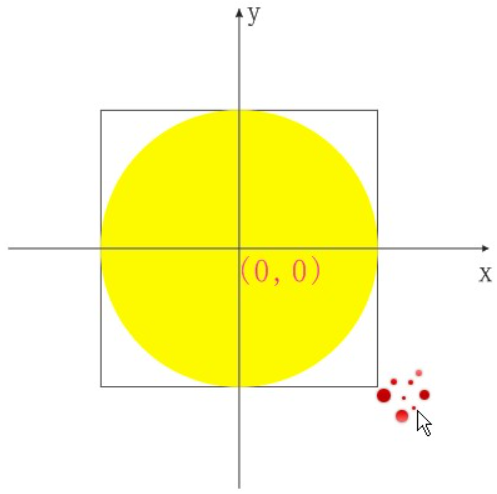
\includegraphics[width=4in,height=4in]{figures/fig1.jpg}
%			\caption{text}
%		\end{figure}
	
	\section{实验目的}
		\begin{itemize}
			\item 
		\end{itemize}
	
	\section{环境配置目的}
		\begin{itemize}
			\item 
		\end{itemize}
	
	\section{实验知识}	
		\begin{itemize}
			\item 
		\end{itemize}
	
	\section{实验要求}
		\begin{itemize}
			\item 
		\end{itemize}
	
	\section{实验环境}
		本次实验实验环境为青椒课堂平台的Linux(Ubuntu 20.04)操作系统。
	
	\section{实验步骤}
	
	
	\section{实验结果截图}	
	
	
	\section{结果分析}
	
	
	\section{困难记录}
	
	
	\section{心得体会}
		做完本次实验,除了掌握了实验目的部分中所有内容的收获之外,我还有以下几点心得体会:
		\begin{itemize}
			\item
		\end{itemize}
	
%\end{sloppypar}
\end{document}
\endinput